\documentclass[10pt]{article}
\usepackage{graphicx}
\usepackage{geometry}
\usepackage{enumerate}
\usepackage{enumitem}
\usepackage{amsmath}
\usepackage[normalem]{ulem}
\usepackage{array}
\usepackage{blkarray} %for block array with external numbering

%1.5 spacing
%\usepackage{setspace}
%\onehalfspacing

%color for code
\usepackage{listings}
\usepackage{color}

\definecolor{dkgreen}{rgb}{0,0.6,0}
\definecolor{gray}{rgb}{0.5,0.5,0.5}
\definecolor{mauve}{rgb}{0.58,0,0.82}

\lstset{frame=tb,
  language=Tcl,
  aboveskip=3mm,
  belowskip=3mm,
  showstringspaces=false,
  columns=flexible,
  basicstyle={\small\ttfamily},
  numbers=none,
  numberstyle=\tiny\color{gray},
  keywordstyle=\color{blue},
  commentstyle=\color{dkgreen},
  stringstyle=\color{mauve},
  breaklines=true,
  breakatwhitespace=true
  tabsize=3
}

%\newcommand{\Problem}[3]{\noindent \textbf{\textbf{Problem #1: {\small #2} [#3 Points] \\ }}}
\newcommand{\Problem}[1]{\noindent \textbf{\textbf{Problem #1:  \\ }}}
\newcommand{\Name}[1]{\noindent \textbf{Name:} #1 \\}
\newcommand{\Workedwith}[1]{\noindent \textbf{Worked with:} #1 \\}
\newcommand{\Solution}{\mbox{} \\ \noindent \textbf{Solution: \\}}
\newcommand{\psheader}[2]{
  \begin{center}{\bf Networks --- CSCI 125, Fall 2014 \\
    Instructors: Goodney \\}
    Lab #1 \\
    Due: 2:00PM on #2
    \vspace*{.5cm}
  \end{center}
}
\newcommand{\DeterLabID}[1]{\noindent \textbf{DETER ID:} #1 \\}
\makeatletter
\newcommand{\thickhline}{%
    \noalign {\ifnum 0=`}\fi \hrule height 1pt
    \futurelet \reserved@a \@xhline
}
\newcolumntype{"}{@{\hskip\tabcolsep\vrule width 1pt\hskip\tabcolsep}}
\makeatother

\begin{document}

%\psheader{HW # HERE}{DUE DATE HERE}
\psheader{3}{Thursday, October 9}


\Name{Bruce Yan (byan@hmc.edu), Angela Zhou (azhou@hmc.edu)}
\DeterLabID{hmc125ah, hmc125-aj}
%\Workedwith{Angela Zhou}

\Problem{1 - Group Project: Fast, Reliable File Transfer}
\texttt{scp}. The `secure copy program' \texttt{scp} is a standard tool on modern UNIX-like machines. It is used to copy files between machines, securely and reliably. However, as we will see, it does not always provide good throughput.
\begin{itemize}
\itemsep0em
\item We created an experiment in DETER with two computers together with a 100Mb/s link and 50ms initial delay.  Below is the .ns file we used.
\begin{lstlisting}
# lab3-part1.ns

# This is a simple ns script. Comments start with #.
set ns [new Simulator]
source tb_compat.tcl

# Define the 4 nodes in the topology
set nodeA [$ns node]
set nodeB [$ns node]

# Define the link and the LAN that connect the nodes
# This sets the link speed between nodeA and nodeB
# There is a 25ms round-trip delay
set link0 [$ns duplex-link $nodeB $nodeA 100Mb 50ms DropTail]

# Set the OS to Ubuntu1204-64-STD (modern)
tb-set-node-os $nodeA FBSD9-64-STD
tb-set-node-os $nodeB FBSD9-64-STD

# Enable routing (static) between all the nodes
$ns rtproto Static

# Instruct the simulator to start
# Go!
$ns run
\end{lstlisting}
\item At the beginning, we did a \texttt{ping} between the two nodes and we received the following delay:
\begin{lstlisting}
64 bytes from 10.1.1.2: icmp_seq=27 ttl=64 time=100.386 ms
64 bytes from 10.1.1.2: icmp_seq=28 ttl=64 time=100.420 ms
64 bytes from 10.1.1.2: icmp_seq=29 ttl=64 time=100.324 ms
64 bytes from 10.1.1.2: icmp_seq=30 ttl=64 time=100.365 ms
\end{lstlisting}
\item Once the experiment started, we used the website to set the delay on the link to zero. The RTT delay between the nodes are now:
\begin{lstlisting}
64 bytes from 10.1.1.2: icmp_seq=31 ttl=64 time=0.324 ms
64 bytes from 10.1.1.2: icmp_seq=32 ttl=64 time=0.358 ms
64 bytes from 10.1.1.2: icmp_seq=33 ttl=64 time=0.387 ms
64 bytes from 10.1.1.2: icmp_seq=34 ttl=64 time=0.302 ms
\end{lstlisting}
\item The average delay appears to be 0.3345 ms.  Using \texttt{iperf -c nodeb -u -p 5001 -b 200M -i 10 -t 60} to test the bandwidth, we have an average of 95.6 Mbits/sec over 6 runs. The Bandwidth delay product is 3.19 Kbits.
\item Explain briefly what the above commands do.  \texttt{dd if=/dev/urandom of=data.bin bs=1m count=200}.  \texttt{dd} is standard linux utility that copies information from stdin to stdout.  Here, \texttt{if} is where we are reading the \texttt{/dev/urandom} file from and we are reading it out to \texttt{of} file called \texttt{data.bin}.  \texttt{bs}, which is the block size of both input and output files, is set to 1 megabyte. \texttt{count} means copy only 200 input blocks.
\item We had to change the ownership on both sides by using the following command: \texttt{sudo chown hmc125ah:HMCCS125 /mnt/data.bin} and \texttt{sudo chown hmc125ah:HMCCS125 /mnt}.  We used the command \texttt{sudo scp data.bin hmc125ah@nodea:/mnt} to copy from nodeB to nodeA.
\item What transfer throughput do you get?  Based on 6 trials, we get a transfer throughput of 11.1MB/s using \texttt{scp}.
\item If we increased the delay from 0ms to 25ms on DETER website, we saw an immediate increase in transfer time.  The average throughput dropped to 900KB/s.  Increasing the delay from 25ms to 75ms on DETER website, the average throughput dropped to be about 300KB/s.  Further increasing the delay from 75ms to 125ms, the throughput dropped to be about 186KB/s.  \texttt{scp} transfer performance seems to degrade quite rapidly.  We tried a variety of \texttt{scp} parameters and they did not seem to have any effect.
\item It does appear that \texttt{scp} has some limitations when transferring file over ssh.  We are guessing that the TCP window size cannot be altered.
\item We graphed the result of the throughput transfer vs loss, which can be seen below. It does not seem too extreme since TCP has to check every packet every time it transfers something.  We believe the reason this happens is because every time data is filled in the TCP window, TCP has the property of auto-checking the integrity of all the packets before sending it off.  If there's significant loss, then the transfer speed will be severely impacted.  \\
$$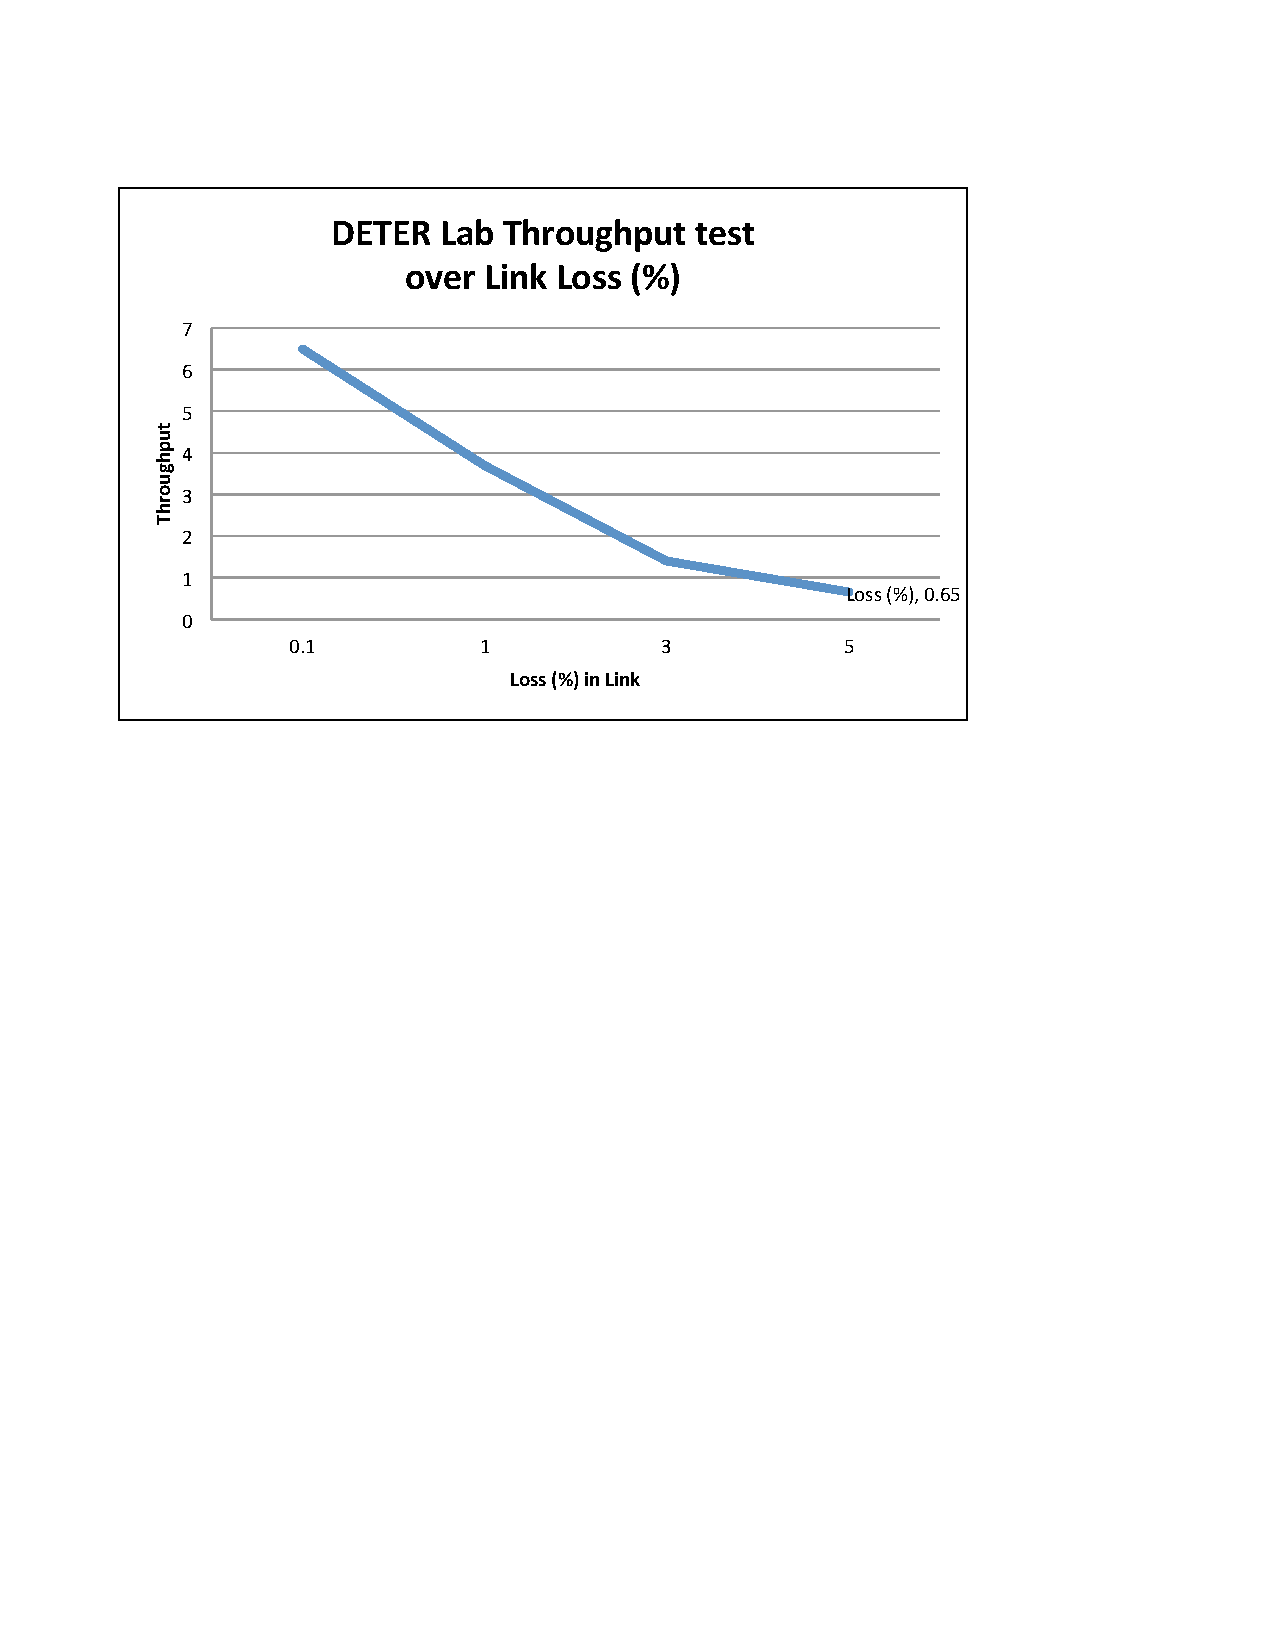
\includegraphics[width=4.5in]{graph-throughput-vs-loss}$$
\item Per Verizon Enterprise Solutions (from Google), the average round-trip transatlantic latency between NY and London is approximately 90ms.  It is also stated that roundtrip latency within North America is 45ms.  Let's just add 30ms of latency for the distance between London and Switzerland.  This total roundtrip is: 165ms.  \\ \\ We would guess the CERN physicist will NOT be asking us for data considering the huge latency.  We could potentially help him, but it would just be slow, considering our CERN physicist friend may need a lot of data.  If we were to help him, we may need another method to transfer files, such as using distributed file systems or Cloud solutions.
\end{itemize}

\newpage


\Problem{2 - File Transfer Utility}
As we've learned above, TCP, while totally reliable and robust, doesn't always give us good throughput. In this section you?ll design a IP based file-transfer utility. The design and implementation of the utility is up to your group, however it must full-fill only three requirements: it must use IP (so it can be routed), it must transfer the file reliably (with no errors) and it must be implemented with a command-line interface similar to \texttt{scp}.

The link speed between the sender and receiver must be \textbf{100Mbps} and the test file size must be at least \textbf{1GBytes}. You should emulate the delay and the loss rate of the link using the delay node. You should test your system under various different conditions. However two settings that you must expose your system for the assignment are:
\begin{itemize}
\itemsep0em
\item The Delay (RTT) of 10ms with the Loss rate of 1\%
\item The Delay (RTT) of 200ms with the Loss rate of 20\%
\end{itemize}
Describe, in detail, the concept(s) behind your file transfer utility, results, and the analysis in the document that must be submitted on October 9th by 2pm. Also, on October 9th and 14th we will have presentations from each group. The presentations will give details on how you solved the problems, problems you encountered and the results you were able to obtain. Some hints:
\begin{itemize}
\itemsep0em
\item There are several closed and open source projects out there that do this. They typically use UDP at their base. You may use them as inspiration, however the end work must be your own. You must use UDP and only UDP for the transport of the file data. However, you may use TCP for control or metadata, but all of the file data, including retransmissions, must use UDP.
\item You can implement the program in any language you'd like (C, C++, Java, Python, Ruby, etc.) as long as it works on the DETER nodes, and your submission comes with clear, concise instructions on how to build and test your program.
\item Think about why \texttt{scp} has issues. Identify these weaknesses as inspiration for solving the problem. Think about selective re-transmission, parallel flows, forward error correction...
\item Learn how to use the following UNIX tools, they are your friends: \texttt{tcpdump, tcpreplay, nc (aka netcat), nmap, netstat, iperf}
\item There will be a prize for the team that achieves the highest throughput on the \textbf{200ms, 20\%} test case!
\item You may need to learn about network programming on UNIX using sockets, and/or \texttt{libpcap}. See: \\
http://beej.us/guide/bgnet/\\
http://www.prasannatech.net/2008/07/socket-programming-tutorial.html\\
http://gnosis.cx/publish/programming/sockets2.html
\item To measure the throughput achieved, the \texttt{time} utility will be used. Familiarize yourself with this utility and understand how to use it to measure the total throughput achieved by your FTP utility.
\end{itemize}



\end{document}